\documentclass[11pt]{article}
\usepackage{natbib,amsmath,amssymb,amsfonts,amsthm,dsfont,enumitem,float}
\RequirePackage[colorlinks,citecolor=blue,urlcolor=blue,breaklinks]{hyperref}
\usepackage[normalem]{ulem}
\usepackage{epsfig,longtable,xcolor,algorithm,algpseudocode}

%%%%%%%%%% page setup %%%%%%%%%%
\textheight 9 in
\textwidth 6.5 in
\topmargin -.5 in
\oddsidemargin 0 in
\renewcommand{\textfraction}{0}
\renewcommand{\floatpagefraction}{0.90}
%Line space
\renewcommand{\baselinestretch}{1.1} 

%%%%%%%%%% define math symbols %%%%%%%%%%
%% bold and cal letters/LETTERS
\newcommand{\bfm}[1]{\ensuremath{\mathbf{#1}}}
\def\ba{\bfm a}     \def\bA{\bfm A}     \def\cA{{\cal  A}}     \def\calA{{\cal  A}}
\def\bb{\bfm b}     \def\bB{\bfm B}     \def\cB{{\cal  B}}     \def\calB{{\cal  B}}
\def\bc{\bfm c}     \def\bC{\bfm C}     \def\cC{{\cal  C}}     \def\calC{{\cal  C}}
\def\bd{\bfm d}     \def\bD{\bfm D}     \def\cD{{\cal  D}}     \def\calD{{\cal  D}}
\def\be{\bfm e}     \def\bE{\bfm E}     \def\cE{{\cal  E}}     \def\calE{{\cal  E}}
\def\bff{\bfm f}    \def\bF{\bfm F}     \def\cF{{\cal  F}}     \def\calF{{\cal  F}}
\def\bg{\bfm g}     \def\bG{\bfm G}     \def\cG{{\cal  G}}     \def\calG{{\cal  G}}
\def\bh{\bfm h}     \def\bH{\bfm H}     \def\cH{{\cal  H}}     \def\calH{{\cal  H}}
\def\bi{\bfm i}     \def\bI{\bfm I}     \def\cI{{\cal  I}}     \def\calI{{\cal  I}}
\def\bj{\bfm j}     \def\bJ{\bfm J}     \def\cJ{{\cal  J}}     \def\calJ{{\cal  J}}
\def\bk{\bfm k}     \def\bK{\bfm K}     \def\cK{{\cal  K}}     \def\calK{{\cal  K}}
\def\bl{\bfm l}     \def\bL{\bfm L}     \def\cL{{\cal  L}}     \def\calL{{\cal  L}}
\def\bm{\bfm m}     \def\bM{\bfm M}     \def\cM{{\cal  M}}     \def\calM{{\cal  M}}
\def\bn{\bfm n}     \def\bN{\bfm N}     \def\cN{{\cal  N}}     \def\calN{{\cal  N}}
\def\bo{\bfm o}     \def\bO{\bfm O}     \def\cO{{\cal  O}}     \def\calO{{\cal  O}}
\def\bp{\bfm p}     \def\bP{\bfm P}     \def\cP{{\cal  P}}     \def\calP{{\cal  P}}
\def\bq{\bfm q}     \def\bQ{\bfm Q}     \def\cQ{{\cal  Q}}     \def\calQ{{\cal  Q}}
\def\br{\bfm r}     \def\bR{\bfm R}     \def\cR{{\cal  R}}     \def\calR{{\cal  R}}
\def\bs{\bfm s}     \def\bS{\bfm S}     \def\cS{{\cal  S}}     \def\calS{{\cal  S}}
\def\bt{\bfm t}     \def\bT{\bfm T}     \def\cT{{\cal  T}}     \def\calT{{\cal  T}}
\def\bu{{\bfm u}}     \def\bU{\bfm U}     \def\cU{{\cal  U}}     \def\calU{{\cal  U}}
\def\bv{\bfm v}     \def\bV{\bfm V}     \def\cV{{\cal  V}}     \def\calV{{\cal  V}}
\def\bw{\bfm w}     \def\bW{\bfm W}     \def\cW{{\cal  W}}     \def\calW{{\cal  W}}
\def\bx{\bfm x}     \def\bX{\bfm X}     \def\cX{{\cal  X}}     \def\calX{{\cal  X}}
\def\by{\bfm y}     \def\bY{{\bfm Y}}     \def\cY{{\cal  Y}}     \def\calY{{\cal  Y}}
\def\bz{\bfm z}     \def\bZ{\bfm Z}     \def\cZ{{\cal  Z}}     \def\calZ{{\cal  Z}}
\def\bzero{\bfm 0}


% \boldsymbol{greek letters}
\newcommand{\bfsym}[1]{\ensuremath{\boldsymbol{#1}}}
\def \balpha   {\bfsym{\alpha}}       \def \bbeta    {\bfsym{\beta}}
\def \bgamma   {\bfsym{\gamma}}       \def \bdelta   {\bfsym{\xi}}
\def \bepsilon {\bfsym{\epsilon}}     \def \bzeta    {\bfsym{\zeta}}
\def \betta    {\bfsym{\eta}}         \def \btheta   {\bfsym{\theta}}
\def \biota    {\bfsym{\iota}}        \def \bkappa   {\bfsym{\kappa}}
\def \blambda  {\bfsym{\lambda}}      \def \bmu      {\bfsym{\mu}}
\def \bnu      {\bfsym{\nu}}          \def \bxi      {\bfsym{\xi}}
\def \bomicron {\bfsym{\omicron}}     \def \bpi      {\bfsym{\pi}}
\def \brho     {\bfsym{\rho}}         \def \bsigma   {\bfsym{\sigma}}
\def \btau     {\bfsym{\tau}}         \def \bupsilon {\bfsym{\upsilon}}
\def \bphi     {\bfsym{\phi}}         \def \bchi     {\bfsym{\chi}}
\def \bpsi     {\bfsym{\psi}}         \def \bomega   {\bfsym{\omega}}
\def \beps     {\bfsym \varepsilon}

% \boldsymbol{GREEK LETTERS}
\def \bGamma   {\bfsym{\Gamma}}       \def \bDelta   {\bfsym{\Delta}}
\def \bTheta   {\bfsym{\Theta}}       \def \bLambda  {\bfsym{\Lambda}}
\def \bXi      {\bfsym{\Xi}}          \def \bPi      {\bfsym{\Pi}}
\def \bSigma   {\bfsym{\Sigma}}       \def \bUpsilon {\bfsym{\Upsilon}}
\def \bPhi     {\bfsym{\Phi}}         \def \bPsi     {\bfsym{\Psi}}
\def \bOmega   {{\bfsym{\Omega}}}


%%%%%%%%%%%%%%%% Regular font in math equation  %%%%%%%
\DeclareMathOperator*{\argmin}{argmin}
\DeclareMathOperator*{\argmax}{argmax}
\DeclareMathOperator{\var}{var}
\DeclareMathOperator{\cov}{cov}
\DeclareMathOperator{\diag}{diag}
\newcommand{\indep}{\perp \hspace{-.25cm} \perp}
\newcommand{\E}{\mathbb{E}}
\DeclareMathOperator{\rank}{rank}
\DeclareMathOperator{\supp}{supp}
\DeclareMathOperator \Tr {\mathrm{tr}}
\DeclareMathOperator \col {\text{Col}}
\DeclareMathOperator \row {\text{Row}}

\def \soft{\text{soft}}
\def \bone   {\bfsym{1}}
\def \RR	{\mathbb{R}}
\def \PP {\mathbb{P}}
\def \SS {\mathbb{S}}
\def \OO {\mathbb{O}}
\def \NN {\mathbb{N}}
\def \vec	{\text{vec}}
\def \mat {\text{mat}}
\def \KL {\text{KL}}


%%%%%%%%%%%%%%%%%%%% self-defined commands go below %%%%%%%%%%%%%%%%%%%%

% Shortcuts to present a math display
\newcommand{\beq}  {\begin{equation}}
\newcommand{\eeq}  {\end{equation}}
\newcommand{\beqn} {\begin{eqnarray}}
\newcommand{\eeqn} {\end{eqnarray}}
\newcommand{\beqnn}{\begin{eqnarray*}}
\newcommand{\eeqnn}{\end{eqnarray*}}

% Colored comments 
\newcommand{\red}[1]{{\color{red}#1}}
\newcommand{\blue}[1]{{\color{blue}#1}}
\newcommand{\orange}[1]{{\color{orange}#1}} 
\newcommand{\teal}[1]{{\color{teal}#1}} 
\newcommand{\zzw}[1]{({\color{blue} Ziwei: #1})}

% Theroems, Definitions, Assumptions, etc. 
\theoremstyle{definition}
\newtheorem{dfn}{Definition}
\newtheorem*{rem}{Remark}
\theoremstyle{plain}
\newtheorem{lem}{Lemma}
\newtheorem{cor}{Corollary}
\newtheorem{prop}{Proposition}
\newtheorem{thm}{Theorem}

% Norms
\providecommand{\abs}[1]{\left\lvert#1\right\rvert}
\providecommand{\norm}[1]{\left\lVert#1\right\rVert}
\newcommand{\lzeronorm}[1]{\lVert#1\rVert_0}
\newcommand{\lonenorm}[1]{\lVert#1\rVert_1}
\newcommand{\ltwonorm}[1]{\lVert#1\rVert_2}
\newcommand{\linfinity}[1]{\lVert#1\rVert_{\infty}}
\newcommand{\opnorm}[1]{\|#1\|_{\mathrm{op}}}
\newcommand{\fnorm}[1]{\|#1\|_{\mathrm{F}}}
\newcommand{\nnorm}[1]{\lVert#1\rVert_*}
\newcommand{\supnorm}[1]{ \lVert#1  \rVert_{\max}}
\newcommand{\twotoinf}[1]{\lVert#1\rVert_{2\rightarrow \infty}}
\newcommand{\onetoone}[1]{\lVert#1\rVert_{1\rightarrow 1}}
\newcommand{\inftoinf}[1]{\lVert#1\rVert_{\infty \rightarrow\infty}}






\title{A useful Latex template}
\author{ABC$^\ast$, DEF$^{\ast,\dagger}$ \\
 \normalsize
 $^\ast$Department of Statistics, University of Michigan \\ \normalsize
 $^\dagger$ Department of ABC, University of DEF \\
\date{\today} }

\begin{document}

\maketitle

\begin{abstract}
  We study an interesting problem in statistics and machine learning. 
\end{abstract}

\section{Main results}

\label{Sec:Proofs}
We define two linear maps $\mathcal{D}, \mathcal{F}: \mathbb{R}^{d\times d}\to \mathbb{R}^{d\times d}$, such that for any $\bA = (A_{ij}) \in\mathbb{R}^{d\times d}$, we have $[\mathcal{D}(\bA)]_{ij} := A_{ij}\mathds{1}_{\{i=j\}}$ and $\mathcal{F}(\bA) := \bA - \mathcal{D}(\bA)$. In other words, $\mathcal{D}(\bA)$ and $\mathcal{F}(\bA)$ correspond to the diagonal and off-diagonal parts of $\bA$ respectively. We write $X \indep Y$ if $X$ and $Y$ are independent. 

\begin{proof}
Define an event
\beq
\cA := \bigl\{\|\widetilde \bW - p^{-2}\bone_d \bone_d^\top\|_\infty \leq p^{-2}\bigr\}.
\eeq
For $j,k\in[d]$, write $\widehat P_{jk} := n^{-1} \sum_{i = 1}^n \omega_{ij}\omega_{ik}$. Then by a union bound and Bernstein's inequality, we have
\[
\PP(\cA^{\mathrm{c}}) \leq \sum_{j,k\in [d]} \PP\bigl(\widehat P_{jk} < p^2/2\bigr) \leq d^2 e^{-3np^2/32}.
\]
Note that on $\cA$, we have $\|\widetilde \bW\|_\infty \leq 2p^{-2}$. The desired bounds then follow respectively from the following inequalities: $\|\widetilde \bW\|_{\mathrm{op}} \leq d\|\widetilde \bW\|_\infty$, $\|\widetilde \bW\|_{1\to 1} = \|\widetilde \bW\|_{\infty\to\infty} \leq d\|\widetilde \bW\|_\infty$, $\|\widetilde \bW\|_1 \leq d^2 \|\widetilde \bW\|_\infty$, $\|\widetilde \bW\|_{\mathrm{F}} \leq d\|\widetilde \bW\|_\infty$ and $\|\widetilde \bW\|_{2\to\infty} \leq d^{1/2}\|\widetilde \bW\|_\infty$. 
\end{proof}

\section{Numerical study}

The simulation shows significant advantage of Method A over Method B. 

\newpage 

Let's make a plot here. Figure \ref{fig:bamboo} compares clipped and original figures. 

\begin{figure}[H]
		\centering
		\begin{tabular}{cc}
		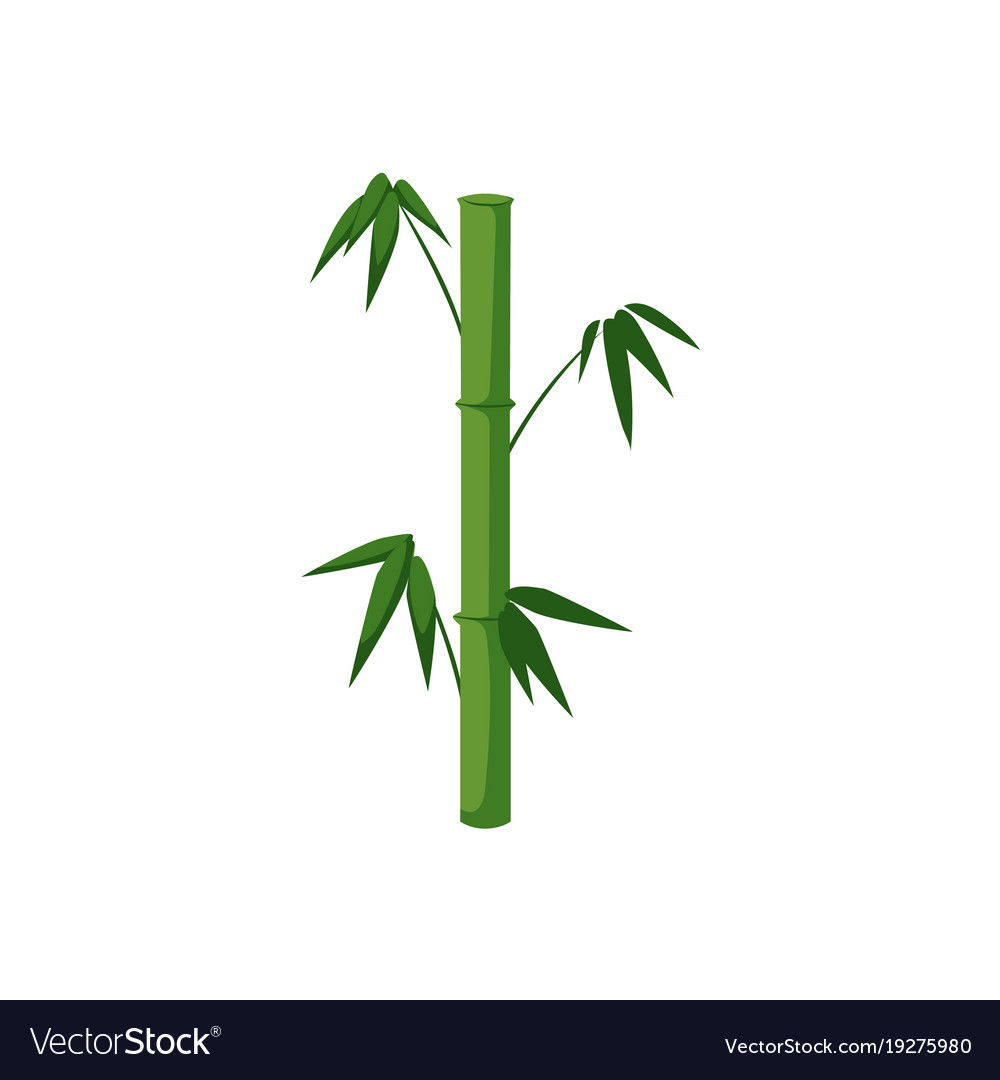
\includegraphics[clip, trim=0 3cm 0 0, scale=.15]{./figs/bamboo}	& 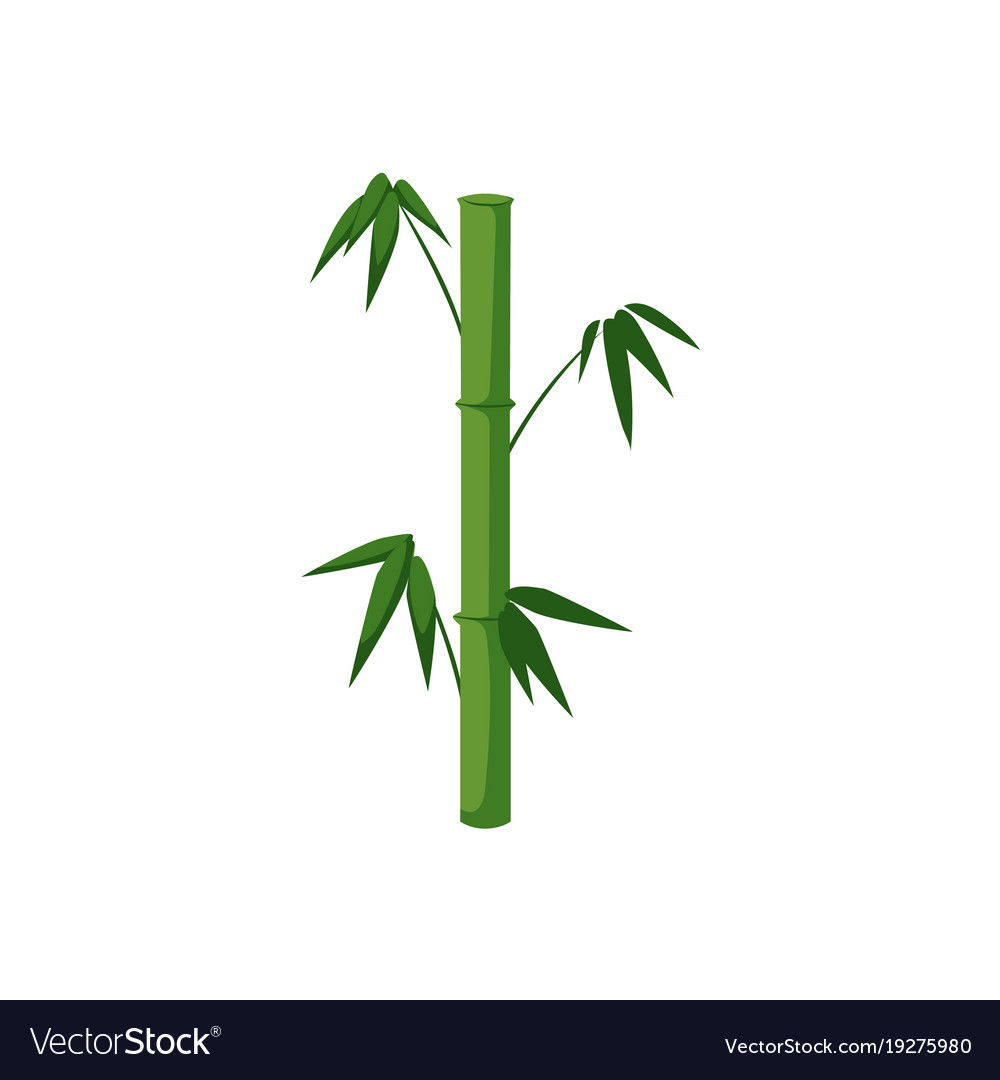
\includegraphics[scale=.15]{./figs/bamboo} \\
		Clipped & Not Clipped
			\end{tabular}
		\vspace{.5cm}
		\caption{Bamboos: Should we clip them or not?}
		\label{fig:bamboo} % Figure labels must be put after the figures so that Latex recognizes it and treats it correctly 
	\end{figure}

Next let's see how we should create tables. 
\begin{table}[H]
	\centering
	\begin{tabular}{cccc}
		\hline\hline
		Methods	& RSS & $\fnorm{\widehat \bTheta - \bTheta ^ *}$ & $\fnorm{\sin\Theta(\widehat \bTheta, \bTheta ^ *)}$ \\ \hline\hline
		IHT & 1.008& 0.018 & 8e-16\\
		Nuclear & 1.006 & 0.033 & 1e-14 \\
		\hline\hline
	\end{tabular}
	\caption{$n = 2000, r = 1, d = 10, k = 1, s = 2, \rho = 0$}	
	\label{tab:unknown}
\end{table}
Table \ref{tab:unknown} is a good-looking table. Finally let's cite some papers. \citet[][]{Oli16} may be too hard for undergrads. \citet[][]{RHu17} is a nice tutorial on high-dimensional statistics. Pay attention to the format of the cite key, with which I hope you can stick. 

\bibliographystyle{ims}
\bibliography{abc}

\end{document}

